\chapter{The GitHub Way}
This chapter describes GitHub in detail, outlining what it is and some of its defining features, how it is used, and why it might be useful in education. GitHub exemplifies `The GitHub Way': an open, collaborative workflow in which users of GitHub and similar platforms work and collaborate, and where one's work is open and available for multiple contributors to edit, add to, and discuss. This is an important distinction as the aim of this work is to investigate not just how GitHub, but also how the underlying activities that GitHub supports can impact education. %as we feel it is not just GitHub itself that can impact education, but rather the activities that GitHub supports.

\section{What is GitHub?}
GitHub is Web-based social code sharing service released in 2008 that utilizes the Git distributed version control system. It is a tool utilized by millions of developers all over the world to facilitate collaboration via the use of its awareness and transparency components, collaborative features such as pull requests, and version control. Some of its primary collaborative features are summarized in \ref{fig:githubfeats}, and described in further detail in this chapter. The tool is organized so that developers can create repositories containing their work, which they develop on their own or share with other developers who can, in turn, contribute to the code. Repositories can be public, which means that anybody can see them and pull the code into their own repositories, though the owner can decide who can and cannot make changes. Alternatively, they can be private, whereby the repository is viewable and editable only by those given permission by the owner.

GitHub recommends repositories to be smaller than 1 GB, and for files to be smaller than 100 MB\footnote{\url{https://help.github.com/articles/what-is-my-disk-quota/}}. Moreover, GitHub recommends hosting file types that contain only plain text, such as code and Markdown files. Markdown is a markup language with plain text formatting designed to be easily convertible to HTML. The language supports text formatting such as headings, lists, and bolded text, and is often the format of `readme' files on GitHub, which typically contain information about the other files in a directory. For example, a project repository's `readme' might contain information such as a description of the project, the programming languages involved, and links to websites relevant to the project.

\begin{figure}[h!]
 \caption{The primary features of GitHub that support collaboration between users.}
 \centering
   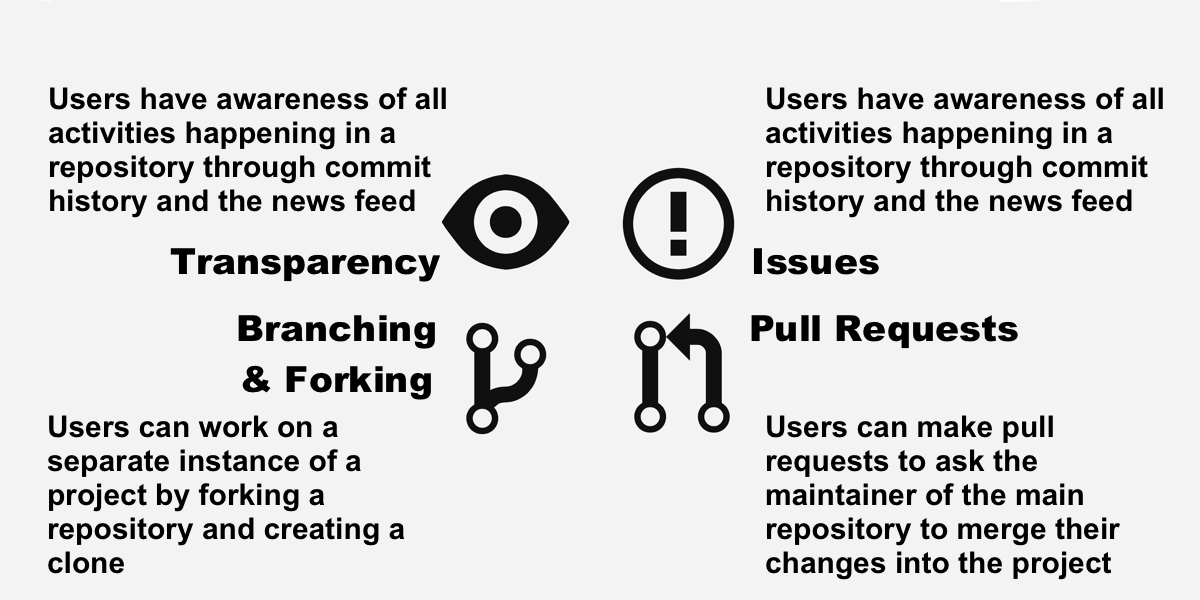
\includegraphics[width=1.0\textwidth]{githubfeats}
 \label{fig:githubfeats}
\end{figure}

\section{Git: Distributed Version Control}
Git is the underlying version control system that GitHub utilizes. There are two very important aspects to Git: that work is distributed, and that work is handled by version control. Being distributed refers to the possibility of work being decentralized: instead of being forced to work in a repository where there is a central hub that everyone pushes code to, individual developers can create public `clones' of that repository and `push' to their respective clones before the original repository's maintainer or owner pulls in the work. This provides many opportunities for remixing and reusing content, as well as supporting a workflow where multiple parties can do separate work at their own pace.

Version control means that developers can easily track changes to their code and that multiple developers can work on the same file, as combining changes requires a simple `merge' process that Git handles. In this system, when a user makes changes to the project, they `commit' their changes, effectively saving a snapshot of the project as it is at that point in time. These commits, or snapshots, are saved in the project's history, allowing developers to revert changes as needed. The user can then push all of their changes to the server, meaning other collaborators can see the changes made. If a collaborator has made changes as well, these can be merged together to combine the different changes into the main code base.

\section{Branching and Forking}
`Branching' and `forking' provides two ways of diverging from the main code base. A user can make changes in a repository `branch', which is a deviation of the code from the code base (the `trunk'), but the changes remain a part of the main repository\footnote{\url{https://guides.github.com/introduction/flow/}}. When a user branches from the trunk, they can still monitor changes to the trunk despite working in a different branch.

`Forking', meanwhile, achieves a similar function of deviating from the code base. The main difference is that a fork is independent of the main code base, meaning a user who forked a repository won't be aware of the changes happening in the main code base unless they are explicitly watching the original repository\footnote{\url{https://help.github.com/articles/fork-a-repo/}}. When a user forks a repository, the repository, including all of its branches, are copied. On the other hand, if a repository is deleted, the fork still exists, a consequence of decentralizing these repositories.

Generally, branching provides a good workflow for development teams whose members need to be aware of all the changes made to each branch and the main code base. Meanwhile, forking tends to work for open-source projects where the repository owner does not want to manage user access to the repository and wants to keep collaborator changes independent until they are ready to be merged.

\section{Merging and Pull Requests}
`Merging' is the mechanism for combining changes or pulling changes from a branch or fork into the main code base. If a user wants to make changes to a repository, they can branch or fork from the main code base and make changes to the code as they see fit, and it would remain in their branch or repository. In order to get changes into the main code base, the person managing the repository (maintainer) would have to merge the changes into it, combining whatever changes were made in the branch or fork with the code base.

`Pull requests' (PRs) are a way of handling these merges. In a PR, the person making the changes in a branch or a fork will request that the code base maintainer merge their code into the main trunk, otherwise known as the master branch. These PRs will be listed on GitHub in a separate tab where collaborators can see each of the commits made, what files were changed, and the conversation surrounding the code. The user making the PR can also add comments to their PR, such as describing their changes or how the changes affect the project or code. Collaborators can also make comments on PRs, typically when changes have to be made before a PR can be accepted, or a `+1' if they think a PR is ready to be merged into the main code base.

In some cases, such as when the same section of code is changed at the same time, `a merge conflict' can occur, which requires the user to manually pick and choose which of the changes or pieces of code they want to keep. However, there can be issues with file types that are not versioned by Git, such as PDF documents or Powerpoint presentations, as changes anywhere in a file within two different branches can create unknown merge conflicts. Moreover, when someone changes a file that is an unsupported file type, collaborators cannot see the changes (the `diff') easily.

\section{Issues and Comments}
The `issues' feature on GitHub provides a mechanism for collaborators to engage in discussion. Issues can be tagged with any label the issue creator or editor wants, such as `bug' or `feature', and the list of issues can be filtered to only show issues that contain a certain tag, or only closed or open issues. Issues can be assigned to a user, letting others know who is in charge of that issue, or they can be assigned to a `milestone', a due date set by a collaborator. PRs are also automatically posted as an issue, which is closed when the associated PR is accepted or closed. Users can comment on issues, making issues a hub for discussion. Users can also refer to issues in commit messages, which links the commit to the issue: for example, an issue fixed by a commit might say \textit{``collaborator closed this in d2ad525 on Oct. 25, 2014.''}

One of GitHub's more important features is the flexibility afforded to users making comments. For example, users can mention others by referring to their username preceded by an `@' character, thereby sending them a notification and, in most cases, an email. This allows collaborators to directly refer to another when, for example, they would like to ask someone to make a specific change to an issue or PR. Users can also comment on more specific artifacts, such as pull requests, commits, or individual lines of code. This gives users the ability to discuss various aspects of a project with other collaborators. For example, when a specific line of code is difficult to understand or causes a bug, that line of code can be highlighted in an issue.

\section{Openness \& Transparency}
GitHub's openness and transparency features allow groups to facilitate both direct and indirect collaboration, allowing users to have a full view of activities occurring in a project. For example, users can look at the commit history and see specific changes on specific commits. This allows them to see exactly what people are working on. This history is useful, and when used with the `blame' feature\footnote{\url{https://help.github.com/articles/using-git-blame-to-trace-changes-in-a-file/}}, shows who changed a specific line of code.

Upon logging into GitHub, the first screen the user will see is their News Feed\footnote{\url{https://help.github.com/articles/news-feed/}}. This displays the activity on all the repositories that the user is involved in or is `watching', a feature described below. Any comments, pushes to code, pull requests, or new issues appear in the News Feed, allowing the user to be aware of the events happening in their repositories.

GitHub also includes the `Watch' feature, which has three options. If a user chooses to `watch' a repository, they will get notifications from any activities in that repository, including changes to the code base, new pull requests, new issues, and comments on PRs, issues, commits, or code. These notifications appear in three potential places: the user's News Feed, as a notification in their Notifications list, and as an email. Alternatively, a user can choose to not watch a repository, meaning they will only be notified if they are specifically mentioned in a comment or commit, or in comment threads that they have participated in. Finally, they can choose to ignore a repository, which will prevent them receiving any notifications for that repository, in any capacity.

The last important feature that promotes openness and transparency is the activity monitor on a repository. On the activity monitor, a user can look at who has contributed to the repository, for example, graphs of number of commits from each person, or lines of code added by each person. As well, numerous features allow a user to get a more wholistic picture of the activity on the repository, such as what time commits are normally made on each day, how each branch is handled in comparison to the master branch, or how many times the repository has been visited\footnote{\url{https://github.com/blog/1093-introducing-the-new-github-graphs}}. Overall, this feature allows a user to see and compare the activity among all collaborators.

\section{Why GitHub for Education?}
Although GitHub has focused on code and project management for software development, other domains that involve collaborative work, such as education \cite{griffin2013github}, have recently begun to take advantage of its features. However, the use of GitHub a different context like education might require instructors to explore alternative teaching and learning activities, or require GitHub to be repurposed to better accommodate teaching activities. Jim Baker, a senior developer and University of Colorado Computer Science lecturer, shared his experiences with GitHub: \begin{quote}\textit{``We had a great experience using GitHub to support a collaborative workflow for the 70+ students in each of the 2 semesters of my CS course.''}\end{quote} He elaborated: \begin{quote}\textit{``Pull requests (PR) are the heart of the GitHub workflow, and we took advantage of PRs, including task lists so that students could report on their work in progress and get over initial humps. Any merged PR got extra credit(!). Because the course had been improved in some way---this seemed like an interesting standard for giving out extra credit. Consequently, we mostly didn't merge PRs for labs, except for bug fixes, but we were always on the lookout for \textbf{better solutions than ours}. PRs were also merged for extra credit, such as \textbf{corrections of my course notes}. Next fall we expect to have \textbf{autograding} implemented as a form of continuous integration, by running against the PRs through postcommit hooks.''}\end{quote}

Other educators have since introduced GitHub into their classrooms and shared their experiences. In 2010, Luis Felipe Borjas\footnote{\url{http://lfborjas.com/2010/10/30/git-classroom-exams.html}} posted about using GitHub organizations\footnote{\url{https://github.com/blog/674-introducing-organizations}}---a way to simplify the management of group-owned repositories---to manage class projects. He also suggested that teachers can use private repositories for exams or homework assignments that students could push to.
%He also applied GitHub to exams: instead of waiting until the exam deadline to upload the exams, students could just \textit{push}\footnote{\url{https://help.github.com/articles/pushing-to-a-remote}} as many times they wished and the last \textit{push} they made before the deadline was going to be considered their final submission.

In 2011, David Humphrey blogged\footnote{\url{http://vocamus.net/dave/?p=1358}} that he asked his students to use Git/GitHub and highly recommended that other instructors do the same. He claimed that although it was a little painful to learn Git/GitHub at the beginning, the payoff would be huge. \textit{``One of the great things about Git in an educational setting is that you don't need to rely on institutional IT, which, in my experience, is never agile enough to help you with revision control. You can put repos on laptops, use USB keys, use DropBox, use GitHub, etc. You don't have to wait for someone to set up a server and make you accounts, don't have to deal with permissions, or any other nonsense that comes with centralized revision control systems.''}

%Version control systems have been used in the classroom as a way of managing students and their work. Reid \& Wilson \cite{Reid:2005:LDI:1047124.1047441} introduced the Concurrent Versions System (CVS) to a second-year computer science course. This provided the instructors with a simple way to manage student assignments, made it easier for students to work in pairs or groups, and gave the instructors a history of student work. Clifton, Kaczmarczyk \& Mrozek \cite{Clifton:2007:SFS:1227504.1227344} used Subversion, another version control system, to collaboratively develop and run introductory computer science courses. The ease of managing courses using Subversion allowed the instructors to free up time from administrative demands, allowing them to spend more time focusing on pedagogical issues. In 2013, Griffin \& Seals used GitHub in the classroom as a version control tool, leveraging the \textit{Branch} and \textit{Merge} features \cite{Griffin:2013:GCJ:2458539.2458551}. When students worked on programming assignments, it was easy to \textit{merge} back into the original project if their version worked, or abandon a branch without destroying the original project.

Apart from these testimonies of using GitHub, as well as other similar, developer-focused tools highlighted in chapter 2, there are now platforms based on the GitHub model that are targeted for education. Created in 2013, Coursefork\footnote{\url{http://coursefork.org/}} is described as \textit{``GitHub for course creation.''}\footnote{\url{http://opensource.com/education/13/9/coursefork-education-tool}} It is a platform for open-sourcing and collaborating on educational material, where educators can upload course materials and allow others to create copies of courses and modify or share them.

Moreover, GitHub has recently launched a portal specifically for using GitHub in education\footnote{\url{https://education.github.com}}, which aims to help both students and educators. Students can apply for an account with free private repositories, while teachers can also apply for an organizational account for their classes, granting them a number of free repositories for students. They also have a student developer pack, which includes free services or discounts from various companies, such as domain hosting or live programming help. Finally, they include a classroom guide where instructors are given guidelines and suggestions for using GitHub to manage their courses, including an example course repository. Given that they released this guide, along with the research where educators are choosing to use GitHub and similar tools for educational purposes, suggests that GitHub may provide numerous benefits to education.
